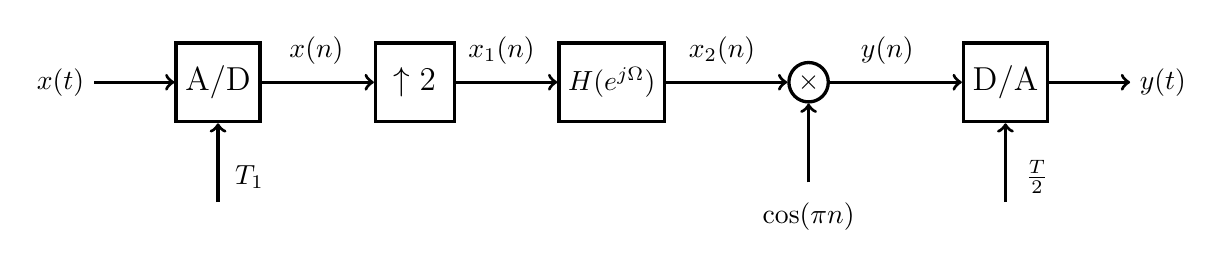
\begin{tikzpicture}[scale=1, transform shape]
    \node[rectangle, very thick, draw, minimum width=1cm, minimum height=1cm] (ad) at (0,0) {\large A/D};
    \node[rectangle, very thick, draw, minimum width=1cm, minimum height=1cm, xshift=2.5cm] (up2) at (ad) {\large $\uparrow 2$};
    \node[rectangle, very thick, draw, minimum width=1cm, minimum height=1cm, xshift=2.5cm] (h) at (up2) {$H(e^{j\Omega})$};
    \node[circle, very thick, draw, inner sep=0.05cm, xshift=2.5cm] (mult) at (h) {$\times$};
    \node[rectangle, very thick, draw, minimum width=1cm, minimum height=1cm, xshift=2.5cm] (da) at (mult) {\large D/A};

    \node[xshift=-2cm] (x_c) at (ad) {$x(t)$};
    \node[xshift=1.25cm,yshift=0.4cm] (x_n) at (ad) {$x(n)$};
    \node[xshift=1.1cm,yshift=0.4cm] (x_1) at (up2) {$x_1(n)$};
    \node[xshift=1.4cm,yshift=0.4cm] (x_2) at (h) {$x_2(n)$};
    \node[xshift=1cm,yshift=0.4cm] (y_n) at (mult) {$y(n)$};
    \node[xshift=2cm] (y_c) at (da) {$y(t)$};
    
    \node[yshift=-1.7cm] (cos) at (mult) {$\cos(\pi n)$};
    \node[yshift=-1.2cm,xshift=0.4cm] (t1) at (ad) {$T_1$};
    \node[yshift=-1.2cm,xshift=0.4cm] (t2) at (da) {$\frac{T}{2}$};

    \draw[->, very thick] (x_c.east) -- (ad.west);
    \draw[->, very thick] (ad.east) -- (up2.west);
    \draw[->, very thick] (up2.east) -- (h.west);
    \draw[->, very thick] (h.east) -- (mult.west);
    \draw[->, very thick] (mult.east) -- (da.west);
    \draw[->, very thick] (da.east) -- (y_c.west);
    \draw[->, very thick] (mult.south) ++ (0,-1cm) -- (mult.south) ;
    \draw[->, very thick] (ad.south) ++ (0,-1cm) -- (ad.south) ;
    \draw[->, very thick] (da.south) ++ (0,-1cm) -- (da.south) ;
\end{tikzpicture}